\section{Calcul du cas à 2 réflexions cas A}
Il a été demandé de calculer l'un des deux cas à 2 réflexions. Le cas ci dessous sera donc étudié.  
\begin{figure}[H]
    \centering
    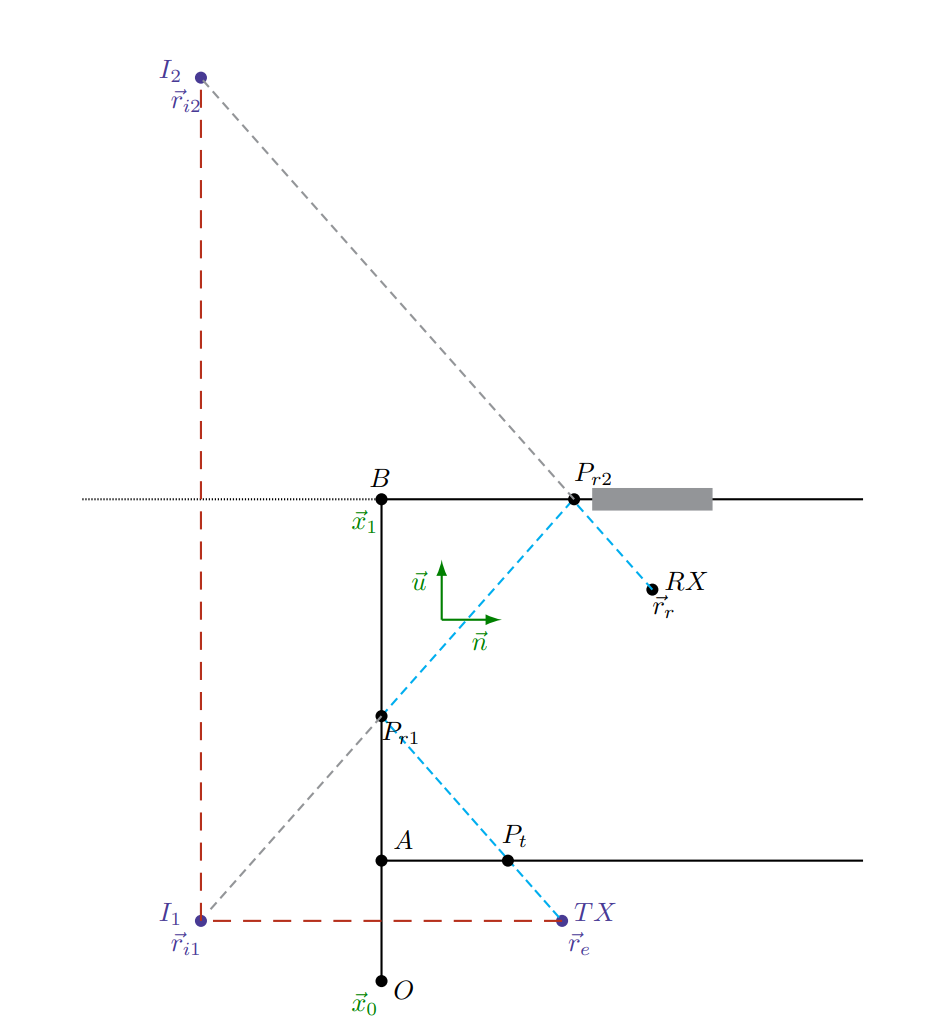
\includegraphics[width=0.58\textwidth]{Pictures/ex41.png}
    \caption{Cas A à 2 réflexions exercice 4.1}
    \label{fig:enter-label}
\end{figure}
\section*{Calcul des positions des points $Pr_2$, $Pr_1$ et $Pt$}

La position des antennes images est déterminée par symétrie orthogonale, avec les coordonnées suivantes pour les antennes images : $I_1 = (-32, 10)$ et $I_2 = (-32, 150)$. Les coordonnées des points $Pr_2$, $Pr_1$ et $Pt$ sont calculées comme suit :


\subsection*{Calcul de $Pr_2$}
$Pr_2$ est un point intermédiaire sur le trajet reliant $I_2$ à $RX$.Pour commencer, le vecteur a été calculé $\vec{v}_1$ entre $I_2$ et $RX$:
\[
\vec{v}_1 = (47 - (-32), 65 - 150) = (79, -85)
\]
La norme de $\vec{v}_1$ est calculée par :
\[
\|\vec{v}_1\| = \sqrt{79^2 + (-85)^2} = 116.0431
\]
Le vecteur unitaire de $\vec{v}_1$ est donc :
\[
\vec{u}_1 = \left(\frac{79}{116.0431}, \frac{-85}{116.0431}\right) = (0.6808, -0.7325)
\]
En posant la coordonnée y de $Pr_2$ à 80, en résolvant pour $\lambda$ dans l'équation suivante :
\[
(y; 80) = (-32; 150) + \lambda \vec{u}_1 \implies \lambda = \frac{80 - 150}{-0.7325} = 95.5631
\]
D'où :
\[
x = -32 + 95.5631 \times 0.6808 = 33.0593
\]
Ainsi, $Pr_2 = (33.0593, 80)$.

\subsection*{Calcul de $Pr_1$}
Pour calculer $Pr_1$, reliant $I_1$ à $Pr_2$, le vecteur $\vec{v}_2$ est :
\[
\vec{v}_2 = (33.0593 - (-32), 80 - 10) = (65.0593, 70)
\]
Sa norme est :
\[
\|\vec{v}_2\| = \sqrt{(65.0593)^2 + 70^2} = 95.5652
\]
Le vecteur unitaire est :
\[
\vec{u}_2 = \left(\frac{65.0593}{95.5652}, \frac{70}{95.5652}\right) = (0.6808, 0.7325)
\]
Pour une coordonnée x de $Pr_1$ à 0, j'ai trouvé $\lambda$ :
\[
(0; y) = (-32; 10) + \lambda \vec{u}_2 \implies \lambda = \frac{0 - (-32)}{0.6808} = 47.0035
\]
Donc :
\[
y = 10 + 47.0035 \times 0.7325 = 44.4301
\]
Finalement, $Pr_1 = (0, 44.4301)$.

\subsection*{Calcul de $Pt$}
La méthode similaire est appliquée pour $Pt$. Le vecteur $\vec{v}_3$ et sa norme sont :
\[
\vec{v}_3 = (0 - 32, 44.4301 - 10) = (-32, 34.4301), \quad \|\vec{v}_3\| = \sqrt{(-32)^2 + (34.4301)^2} = 47.0046
\]
Le vecteur unitaire est :
\[
\vec{u}_3 = \left(\frac{-32}{47.0046}, \frac{34.4301}{47.0046}\right) = (-0.6808, 0.7325)
\]
Pour une coordonnée y de $Pt$ à 20, $\lambda$ est résolu comme suit :
\[
(x; 20) = (32; 10) + \lambda \vec{u}_3 \implies \lambda = \frac{20 - 10}{0.7325} = 13.6519
\]
Ce qui donne :
\[
x = 32 + 13.6519 \times (-0.6808) = 22.7058
\]
Ainsi, $Pt = (22.7058, 20)$.

\section*{Coefficients de réflexion et transmission}

Le rayon subit une transmission et deux réflexions au cours de son trajet. Il est donc nécessaire de calculer deux coefficients de réflexion ainsi qu'un coefficient de transmission.

\subsection*{Calcul du coefficient $\Gamma_2$}
Le vecteur normal au point $Pr_2$ est donné par $(0, -1)$. La projection de $\vec{v}_1$ normé sur ce vecteur normal donne $\cos \theta_i = \langle (0.6808, -0.7325), (0, -1) \rangle = 0.7325$. Ainsi, $\sin \theta_i$ est obtenu par:
\[
\sin \theta_i = \sqrt{1 - 0.7325^2} = 0.6808.
\]
Le $\sin \theta_t$ est déterminé par la loi de Snell:
\[
\sin \theta_t = \sqrt{\frac{1}{\epsilon_r}} \sin \theta_i = \sqrt{\frac{1}{4.8}} \times 0.6808 = 0.3107 \quad \text{et donc} \quad \cos \theta_t = \sqrt{1 - 0.3107^2} = 0.9505.
\]
La distance de pénétration $s$ est calculée comme:
\[
s = \frac{l}{\cos \theta_t} = \frac{0.15}{0.9505} = 0.1578.
\]
Le coefficient de réflexion $\Gamma_{\perp}$ est alors:
\[
\Gamma_{\perp} = \frac{Z_m \cos \theta_i - Z_0 \cos \theta_t}{Z_m \cos \theta_i + Z_0 \cos \theta_t} = \frac{(171.57 + j6.65) \times 0.7325 - 377 \times 0.9505}{(171.57 + j6.65) \times 0.7325 + 377 \times 0.9505} = -0.4805 + j0.0149.
\]
Avec ces valeurs, $\Gamma_2$ est calculé par:
%\Gamma_m(\theta_i) = \Gamma_{\perp}(\theta_i) - \frac{(1 - \Gamma^2_{\perp}(\theta_i)) \Gamma_{\perp}(\theta_i) e^{-2\gamma_m s} e^{j\beta2s \sin \theta_t \sin \theta_i}}{1 - \Gamma^2_{\perp}(\theta_i) e^{-2\gamma_m s} e^{j\beta2s \sin \theta_t \sin \theta_i}}

\[
\Gamma_2 =  \Gamma_{\perp}(\theta_i) -(1 - \Gamma^2_{\perp}(\theta_i)) \frac{ \Gamma_{\perp}(\theta_i) e^{-2\gamma_m s} e^{j\beta2s \sin \theta_t \sin \theta_i}}{1 - \Gamma^2_{\perp}(\theta_i) e^{-2\gamma_m s} e^{j\beta2s \sin \theta_t \sin \theta_i}} = -0.4188 + 0.2462j.
\]

\subsection*{Calcul du coefficient $\Gamma_1$}
Pour le deuxième calcul, je projete $\vec{v}_2$ normé sur la normale $(1, 0)$, donnant $\cos \theta_i = 0.6808$. Les calculs suivants utilisent cette valeur:
\[
\sin \theta_i = 0.7325, \quad \sin \theta_t = 0.3343, \quad \cos \theta_t = 0.9425, \quad s = 0.1591.
\]
Le coefficient de réflexion perpendiculaire $\Gamma_a$ est:
\[
\Gamma_{a,\perp} = \frac{Z_m \cos \theta_i - Z_0 \cos \theta_t}{Z_m \cos \theta_i + Z_0 \cos \theta_t} = \frac{(171.57 + j6.65) \times 0.6808 - 377 \times 0.9425}{(171.57 + j6.65) \times 0.6808 + 377 \times 0.9425} = -0.5050 + j0.0144.
\]
Ainsi, $\Gamma_1$ est:
\[
\Gamma_1 = \Gamma_{\perp}(\theta_i) -(1 - \Gamma^2_{\perp}(\theta_i)) \frac{ \Gamma_{\perp}(\theta_i) e^{-2\gamma_m s} e^{j\beta2s \sin \theta_t \sin \theta_i}}{1 - \Gamma^2_{\perp}(\theta_i) e^{-2\gamma_m s} e^{j\beta2s \sin \theta_t \sin \theta_i}}= -0.4710 + 0.2518j.
\]

\subsection*{Calcul du coefficient de transmission $T_1$}
Le $\cos \theta_i$ pour le point $Pt$ est $0.7325$. En dérivant $\sin \theta_i$, $\sin \theta_t$, et $\cos \theta_t$ comme précédemment. Le coefficient de réflexion perpendiculaire $\Gamma_b$ est:
\[
\Gamma_{b,\perp} = \frac{Z_m \cos \theta_i - Z_0 \cos \theta_t}{Z_m \cos \theta_i + Z_0 \cos \theta_t} = \frac{(171.57 + j6.65) \times 0.7325 - 377 \times 0.1578}{(171.57 + j6.65) \times 0.7325 + 377 \times 0.1578} = -0.5082 + j0.0144.
\]
Le coefficient de transmission $T_1$ est alors calculé par:
\[
T_1 = \frac{ (1 - \Gamma^2_{\perp}(\theta_i)) e^{-2\gamma_m s}}{1 - \Gamma^2_{\perp}(\theta_i) e^{-2\gamma_m s} e^{j\beta2s \sin \theta_t \sin \theta_i}} = 0.6295 + 0.0890j.
\]

%\section*{Calcul de la distance totale parcourue par le rayon et puissance reçue au récepteur}

%\subsection*{Distance totale parcourue par le rayon}
%La distance totale parcourue par le rayon est calculée en additionnant les distances entre les différents points du trajet du rayon de $TX$ à $RX$ :
%\begin{align*}
%\text{Trajet } TX/Pt & : \sqrt{(22.7058 - 32)^2 + (20 - 10)^2} = 13.6522, \\
%\text{Trajet } Pt/Pr1 & : \sqrt{(0 - 22.7058)^2 + (44.4301 - 20)^2} = 33.3524, \\
%\text{Trajet } Pr2/Pr1 & : \sqrt{(33.0593 - 0)^2 + (80 - 44.4301)^2} = 48.5606, \\
%\text{Trajet } PRX/Pr2 & : \sqrt{(47 - 33.0593)^2 + (65 - 80)^2} = 20.4779.
%\end{align*}
%La distance totale est donc de $116.0431$ mètres. Cette distance peut également être vérifiée en calculant directement la distance entre la dernière antenne image $I_2$ et le récepteur $RX$ :
%\[
%\sqrt{(47 - (-32))^2 + (65 - 150)^2} = 116.0431 \text{ mètres}.
%\]

\subsection{Calcul du champ et de la puissance reçue au récepteur}
La valeur du champ électrique reçu, $E_n$, est calculée à partir des coefficients de transmission et de réflexion, et est donnée par :
\[
E_n = \Gamma_1 \Gamma_2 T_1 \sqrt{60 G_{TX} P_{TX}} \frac{e^{-j \beta d_n}}{d_n}
\]
où $\Gamma_1 = -0.4710 + 0.2518j$, $\Gamma_2 = -0.4188 + 0.2462j$, $T_1 = 0.6295 + 0.0890j$, et $d_n = 116.0431$(norme de $v_1$). En calculant $\Gamma_1 \Gamma_2 T_1$ :
\[
\Gamma_1 \Gamma_2 T_1 = (-0.4710 + 0.2518j)(-0.4188 + 0.2462j)(0.6295 + 0.0890j) = 0.1059 - 0.1273j
\]
Ainsi, en substituant les valeurs et calculant $\beta$ à partir de la fréquence $f = 868.3$ MHz :
\[
\beta = \frac{2\pi f}{c} = \frac{2\pi \times 868.3 \times 10^6}{3 \times 10^8} \quad (\text{avec } c \text{ la vitesse de la lumière})
\]
La valeur de $E_n$ obtenue est :

\[
E_n = (0.0159 - 0.1273j) \sqrt{60 \times 1.64 \times 10^{-3}} \frac{e^{-j \beta \times 116.0431}}{116.0431} 
\]
\[
E_n \approx 4.4519 \times 10^{-4} - 2.1816 \times 10^{-5}j
\]
La puissance totale reçue, $P_{RX}$, est ensuite calculée par :
\[
P_{RX} = \frac{\lambda^2}{8\pi^2 R_a} \|E_n\|^2 = \left(\frac{3 \times 10^8}{868.3 \times 10^6}\right)^2 \frac{1}{8\pi^2 \times 73} \|4.4519 \times 10^{-4} - 2.1816 \times 10^{-5}j\|^2
\]
\[
P_{RX} \approx 4.1145 \times 10^{-12} \text{ Watts} \quad \text{ou} \quad P_{RX} \approx -83.8568 \text{ dBm}
\]
\begin{table}[htbp]
\centering
\caption{Comparaison des résultats manuels et simulés pour la réflexion doubles cas A}
\label{tab:double_reflection_comparison}
\begin{tabular}{@{}lcc@{}}
\toprule
\textbf{Paramètre} & \textbf{Valeur Manuelle} & \textbf{Valeur de Simulation} \\ \midrule
Point d'impact 1 & $(0, 44.4301)$ & $(0.0, 44.4304)$ \\
Point d'impact 2 & $(33.0593, 80)$ & $(33.059, 80.0)$ \\
Angle d'incidence($\Gamma_1$) $\theta_{i1}$ (degrés) & $47.09381$ & $47.09525256$ \\
Angle de transmission $\theta_t1$ (degrés) & $19.531$ & $19.531971$ \\
Angle d'incidence($\Gamma_2$) $\theta_{i2}$ (degrés) & $42.9031$ & $42.90474743$ \\
Angle de transmission $\theta_t2$ (degrés) & $18.103$ & $18.1034009$ \\
Coefficient de réflexion $\Gamma_{\perp1}$ & $(-0.5050+0.0144j)$ & $(-0.504537+0.014614j)$ \\
Coefficient de réflexion $\Gamma_{\perp2}$ & $(-0.4805+0.0149j)$ & $(-0.480021+0.014929j)$ \\
Coefficients de transmission 1 & $(0.6295+0.0890j)$ & $(0.6289223+0.0918245j)$ \\
Coefficients de transmission 2 & $1.0$ & $1.0$ \\
Coefficients de transmission 3 & $1.0$ & $1.0$ \\
Distance totale (mètres) & $116.0431$ & $116.043095$ \\
Coefficient total & $(0.1059-0.1273j)$ & $(0.1064106-0.1273762j)$ \\
Champ électrique (V/m)& $4.4519 \times 10^{-4} - 2.1816 \times 10^{-5}j$ & $(3.05628 \times 10^{-5} - 0.0004476j)$  \\
Puissance reçue (W)&$4.1145 \times 10^{-12}$ & $4.16327 \times 10^{-12}$  \\

\bottomrule
\end{tabular}
\end{table}